% !TEX root = ../proj_report_outline.tex

\chapter{Evaluation of architectures}\label{C:exps}
In this chapter we present experimental results comparing the performance of the proposed architectures.
The goal is two-fold: firstly we want to verify the feasibility and ease of use of the models, secondly
we want to see if they achieved the goal of improving on existing architectures. The first goal is
important as the architectures introduce a new hyper-parameter, the tensor rank, and we need to see if
this is a significant hindrance to using the models in practice. The second is equally important, as no
matter how appealing and conceptually grounded the architectures are, they are not useful if they do
not perform in the real world.

Initialisation of the various architectures was not explored in great detail. For most networks we
find initialising the square matrices to be orthonormal and sampling others from a small uniform
distribution is a sufficiently robust procedure. A brief explanation of how random orthonormal
matrices are sampled, as well as a visual comparison of some procedures can be found in
appendix~\ref{A:init}.

\section{Synthetic Tasks}
The synthetic tasks are designed to be highly difficult. Most synthetic tasks for RNNs explored in
the literature have focused on long time dependencies. While these provide a useful measure of the
stability of a model's memory, we also wish to determine how capable a model is at using its memory to
read and write arbitrary patterns. To do this we have had to propose a new synthetic task which identifies
key weaknesses in the LSTM and GRU which are resolved by the TGU. As the tasks in this section are
highly pathological, we do not report results for Vanilla RNNs or the GMR as they are unable to resolve
the time dependencies required.

\subsection{Addition}\label{sec:addition}
\subsubsection{Task}
This task is designed to test the networks' ability to store information for long time periods. It first
featured in \autocite{Hochreiter1997}, although we use the slightly different formulation found more 
recently in \autocite{Le2015}. The problem is a common benchmark for RNNs and has featured in a number of
recent works (\autocite{Arjovsky2015, Henaff2016, Barone2016, Neyshabur2016} for example).

The inputs for this task are sequences of \(T\) pairs. One element of the input is sampled from a uniform
distribution over the range \([0,1]\) while the other is zero except for two locations where it is one.
The location of the first one is always chosen to be earlier than \(T/2\) while the second is after.
The goal is to output at the last time step the sum of the two random values that were presented when the
second input was one. Pseudocode for an algorithm to generate sequences is presented in the appendix,
section~\ref{sec:additionpseudo} while figure~\ref{fig:additionpics} shows an example.
This task becomes harder as the \(T\) increases because the length of time the numbers have to
be remembered for increases.

\subsubsection{Experiment Setup}
We test a number of architectures on sequences with \(T\) of \(250, 500\) and \(750\). As we are
concerned purely with the ability of the networks to solve the task, we generate a new batch of
sequences at each step. All models were allowed \(8\) hidden units and trained on batches of \(8\)
data items to minimise the squared error between the output of the network at the final time step and
the target value. The TGU was allowed a rank \(4\) tensor, giving it the smallest number of parameters
of the gated architectures tested.
Updates were applied using ADAM \autocite{Kingma2014} with a base learning rate chosen
from \(\{0.1, 0.01, 0.001, 0.0001\}\) according to speed of convergence. For all runs, training continued
for \(1800\) updates. While some authors have found they require significantly more updates for success
with certain architectures (up to 10,000,000 in the case of \autocite{Le2015}) we found most successful
architectures converge within 500 on most sequences.

While previously reported results for this task stop at \(T=750\), our most successful architectures still
converge rapidly to a solution at this length. In order to more fully test the limits we increase
\(T\) to 1,000, 5,000 and 10,000. The same parameters were used but only the architectures tested that
were able to solve the task at \(T=750\) were applied to these much more challenging tasks. In order
to reliably find solutions at length 10,000 we had to increase the number of hidden units to \(32\), the
rank of the tensor decomposition was increased proportionally to \(16\).

The models tested were the LSTM, GRU, IRNN \autocite{Le2015} and our TGU. 
For the TGU we separate the bias matrices and use a layer of ReLUs for the candidate
production. All models use a linear output layer to reduce the hidden states back to a scalar prediction.

\subsubsection{Results}
The baseline for this task is a mean squared error of \(0.1767\) which corresponds to predicting
\(1\) for every input sequence.
Figure~\ref{fig:addresults} shows that we were unable to find a solution with the IRNN or LSTM within
the time allotted, while the GRU and TGU consistently did so very rapidly -- in less than 1,000
iterations which is several orders of magnitude faster than previously published results 
\autocite{Le2015, Arjovsky2015, Henaff2016}.

The figures also show that this task can be somewhat frustrating. Due to the online nature, the loss
curves are very noisy, so it is almost impossible to determine whether a model is making progress.
In accordance with a number of others' results \autocite{Le2015, Arjovsky2015} many
architectures will sit on or around the baseline showing no signs of progress for thousands of
training steps before suddenly and rapidly converging to a solution, such as
the GRU on sequence length 1000 in figure~\ref{fig:addlong}. 
We have refrained from smoothing the loss curves to make clear this abrupt shift in behaviour when models begin
to converge.

\begin{figure}[ht]
\centering
\begin{subfigure}[t]{0.75\textwidth}
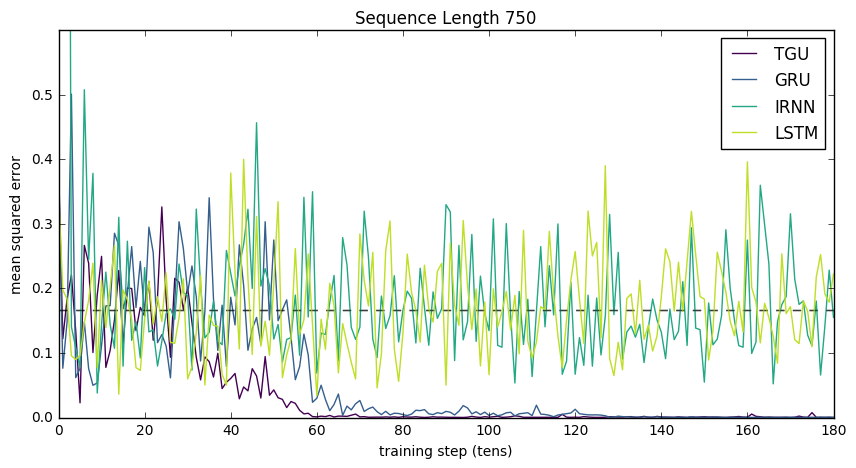
\includegraphics[width=\textwidth]{exps/addition/sl750}
\caption{Sequence length 750.}
\label{fig:add750}
\end{subfigure}

\begin{subfigure}[t]{0.75\textwidth}
\centering
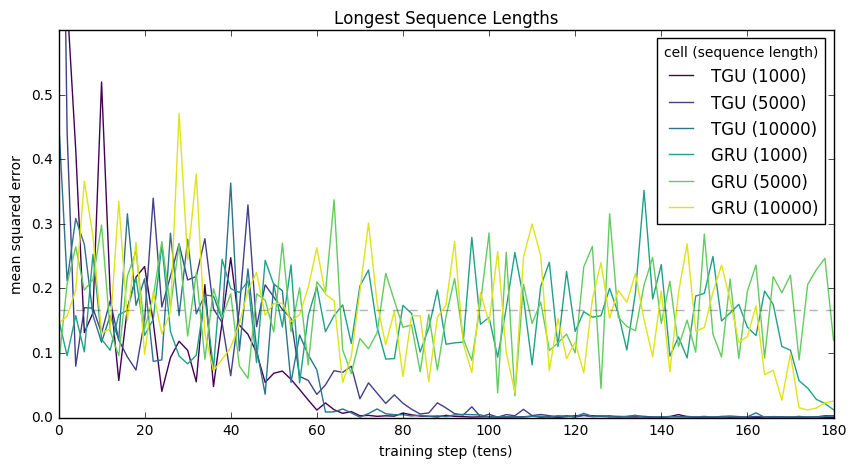
\includegraphics[width=\textwidth]{exps/addition/long}
\caption{Very long sequences.}
\label{fig:addlong}
\end{subfigure}

\caption{Results for addition task}
\label{fig:addresults}
\end{figure}

On sequences up 750 steps, there is little to separate the GRU and the TGU. As they share a gating
mechanism, it is probable that this is a key factor in their success. As discussed in
chapter~\ref{C:arch} this convex gating mechanism is naturally capable of representing exactly the
behaviour required to solve this task -- remembering precisely a small subset of inputs.


Although the convex gate is excellent at picking out individual time steps to remember, it still
has the character of an exponential decay, especially from random initialisation. However, 
we were unable to find a sequence too long for the TGU. 
Results for the TGU and GRU on long sequences are shown in 
figure~\ref{fig:addlong}. The GRU begins to beat the baseline on two of the
tasks inside 2,000 updates. More remarkably, the TGU seems almost completely unaffected by the
extreme length of the sequences still achieving a solution inside 1,000 steps.

We found that the TGU performed much better on this task with a ReLU layer producing candidate updates,
which is contrary to findings on several later tasks.
A possible reason for this is that it is very easy for the ReLU layer to output exactly \(0\).
If the candidate activation mechanism is able to learn to simply output zeros when the appropriate
input is zero, then if the gate is able to stay constant the task is essentially solved -- there should
be at least one hidden unit that will contain a value proportional to the correct answer. Therefore,
we would expect all gated units with an additive state update to perform excellently on this task, those
with a rectified state update only more so.

For the sequences with length 10,000 the expected time dependency (the number of steps between the
two inputs the network has to remember) is 5,000. The network then has to preserve this value in its
memory for an average of 2,500 steps. If we consider taking the RNN and unrolling it across all 10,000
time steps, it is equivalent to a feed-forward network of extraordinary depth and shared weights at each
layer.\footnote{As the error is only computed on the final output for this task, the analogy is very
close -- the RNN is precisely a deep feed-forward network with shared weights and additional inputs
at each layer.} In order to train it successfully we must back-propagate gradients through
7,500 steps on average. While the shared weights undoubtedly assist greatly it is worth observing that this
is still more than 5 times the depth of the deepest feed-forward networks reported
\autocite{Huang2016}.

These results reveal a key weakness in the LSTM. While others have shown 
it is capable of solving the task eventually \autocite{Henaff2016}, it was unable to do so in a comparable
number of training steps.
This adds weight to the hypothesis that the co-operation required between components in the LSTM 
is challenging to learn by gradient descent.

\subsection{Variable Binding}
This task is designed to test the architectures' ability to store arbitrary patterns in memory and
recall them in an organised manner. We term this ``variable binding'' as to solve the task the network needs
to be capable of associating an arbitrary value with a specific label. This task is a natural
sub-task of many large scale problems to which RNNs have already been successfully applied.
An example is translation -- in an end-to-end translation system, the network must perform tasks such
as detecting subjects and objects of sentences, store them appropriately and reproduce them at an
arbitrary time.

Curiously, we could not find a satisfactory task in the literature which tested this ability.
Close alternatives include
the copy task in \autocite{Hochreiter1997} and the variants considered in \autocite{Graves2014}, but these
are concerned with recalling the order in which symbols from a fixed vocabulary appear. 
The ``variable assignment'' task
used to evaluate the Associative LSTM \autocite{Danihelka2016} has a similar aim in mind but again
assesses recall of temporal patterns which does not require learning the kind of delayed one-to-one
mapping we want to investigate.

\subsubsection{Task}
We propose the following synthetic task to test the ability of the network to learn this sort of
mapping: inputs and targets are sequences of length \(T\). Inputs at each time step are
binary vectors of size \(D+N\). The first \(D\) elements of the input are the ``pattern bits'' while
the remaining \(N\) are the ``label bits''. \(N\) different binary patterns are presented to the
network at randomly chosen time steps in the first half of the sequence, the pattern bits are zero at
all other times. Immediately before a pattern is presented, one of the label bits is set. The label
bit is then held until a randomly chosen time step where it is cleared.
At this point, the network must output the corresponding pattern. Label bits are never reused. The target
sequence to match consists of vectors of size \(D\), containing the appropriate pattern at the moment each
of the label bits switches off and zeros elsewhere. Section~\ref{sec:vbinddata} in the appendix includes
some examples of this
while algorithm~\ref{alg:vbinddata} in the appendix demonstrates how to produce appropriate data.

This task involves a number of interesting concepts. A correct solution will need to learn a
transformation from input patterns to hidden states and then learn the inverse transform
to produce the correct output. The requirement of invertibility suggests a reason
for the success of the TGU with linear candidate updates, as the correct output can be reconstructed
by applying the inverse lienar transformation, which may be easier to learn than the inverse of a
highly non-linear transformation. Storing and recalling multiple distinct items also 
requires the ability to be selective about updating the hidden state, which suggests gated architectures
should perform well.

\subsubsection{Experiment Setup}
For this task we found the same hyper parameters to be robust for all models.
Models were trained with a batch size of \(32\) using ADAM with a base learning rate of \(0.01\).
We ceased training after 5000 steps --  although some models were only just beginning to learn
by this time, it is sufficient to see the difference in how easily they are able to arrive
at a solution.

As the targets are binary vectors we use a sigmoid output layer and train to minimise the
sum of the cross entropy at each output at each time step.
For all results reported we use eight bit patterns and test on sequences of length 100, 200 and 500
with one, two and three patterns leading to nine different experiments.

The baseline behaviour, which all architectures achieved rapidly,
is to wait until any of the label bits turns off and output a pattern with mean 0.5. This
achieves a total loss on sequences with \(N\) eight bit patterns of \(-8N\log 0.5\).
Examples of a networks exhibiting this behaviour can be found in figure~\ref{fig:vbindfail}
in the appendix.

As the aim is to assess the ability of the networks to solve the task, we train in an online
fashion. This means that rather than generate a training and test set, we generate new sequences
as required and only report the training error as in this case it is equivalent to generalisation
performance.

We set the number of hidden units to ten times the number patterns to remember for each architecture.
This leads to considerable difference in the number of parameters, but this task is primarily
concerned with the ability of an RNN to use its memory sensibly, so it is fair to ensure they
all have the same quantity of memory. As the patterns are eight bits, having ten hidden units
per pattern ensures it is possible for the networks to store the inputs directly and still have
some units to track the label bits. As the patterns are binary, it should be
straightforward to learn a compressed representation, so these networks are very much overspecified.

\subsubsection{Results}
We report results for the LSTM, GRU, IRNN and TGU. For the TGU we incorporate the biases into
the decomposition (we denote this TGU-C) and use linear activations which was found to give the
most consistent results. We also tested the Vanilla RNN, which was unable to beat the baseline in
any tests and several TGU variants -- for clarity we only present the results of architectures which
showed at least some promise. We were unable to reliably train IRNNs on sequences longer than
100, despite heavy gradient clipping the gradients
consistently exploded. Therefore we only report IRNN results on
the tasks with length 100. We show the median of five runs as there were occasional outliers.

\begin{figure}[tbh]
\centering
\begin{subfigure}[t]{0.3\linewidth}
	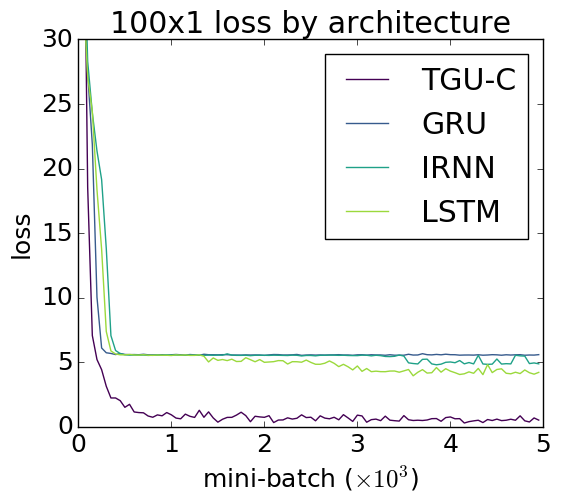
\includegraphics[width=\linewidth]{exps/vbind/plots/100x1}
	\caption{Sequence length 100.}
\end{subfigure}~
\begin{subfigure}[t]{0.3\linewidth}
	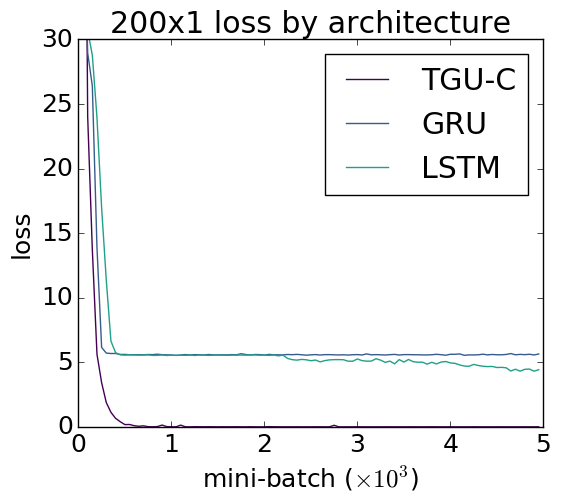
\includegraphics[width=\linewidth]{exps/vbind/plots/200x1}
	\caption{Sequence length 200.}
\end{subfigure}~
\begin{subfigure}[t]{0.3\linewidth}
	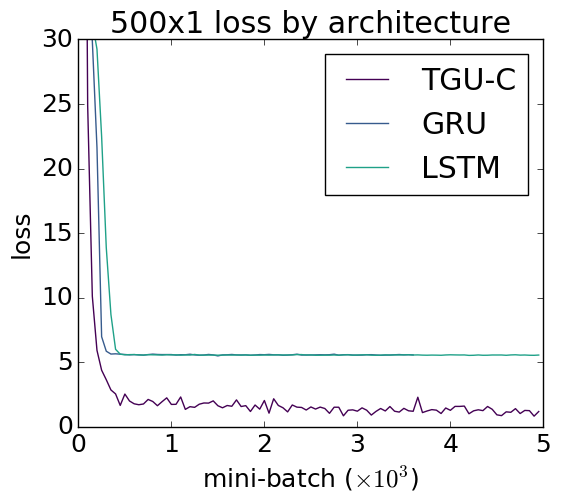
\includegraphics[width=\linewidth]{exps/vbind/plots/500x1}
	\caption{Sequence length 500.}
\end{subfigure}

\caption[Variable binding results, one pattern]
{Variable binding results for sequences containing \(1\) pattern to remember. The baseline loss for this
task is 5.5452.}
\label{fig:vbindn1}
\end{figure}

\begin{figure}[htb]
\centering
\begin{subfigure}[t]{0.3\linewidth}
	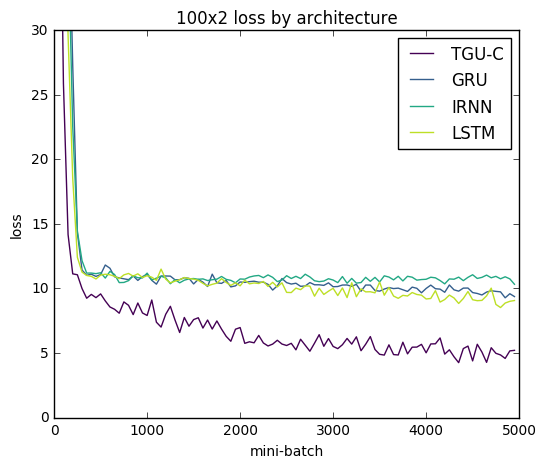
\includegraphics[width=\linewidth]{exps/vbind/plots/100x2}
	\caption{Sequence length 100.}
\end{subfigure}~
\begin{subfigure}[t]{0.3\linewidth}
	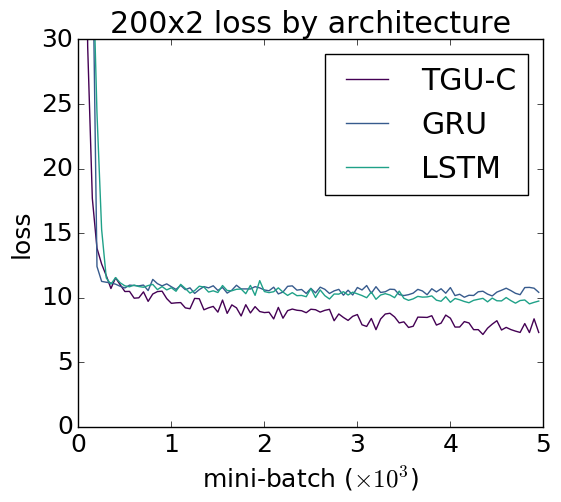
\includegraphics[width=\linewidth]{exps/vbind/plots/200x2}
	\caption{Sequence length 200.}
\end{subfigure}~
\begin{subfigure}[t]{0.3\linewidth}
	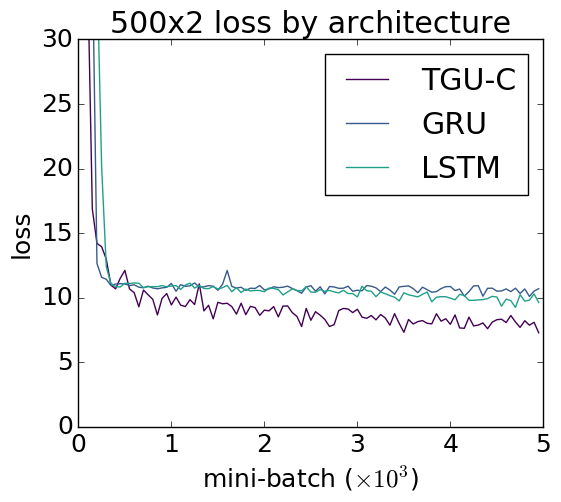
\includegraphics[width=\linewidth]{exps/vbind/plots/500x2}
	\caption{Sequence length 500.}
\end{subfigure}

\caption[Variable binding results, two patterns]
{Variable binding results for sequences containing \(2\) patterns to remember. The baseline loss for this
task is 11.0904.}
\label{fig:vbindn2}
\end{figure}

\begin{figure}[htb]
\centering
\begin{subfigure}[t]{0.3\linewidth}
	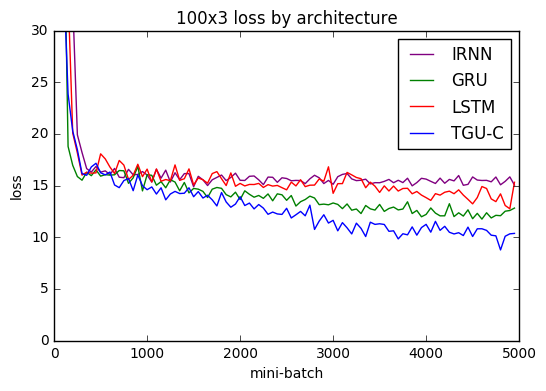
\includegraphics[width=\linewidth]{exps/vbind/plots/100x3}
	\caption{Sequence length 100.}
\end{subfigure}~
\begin{subfigure}[t]{0.3\linewidth}
	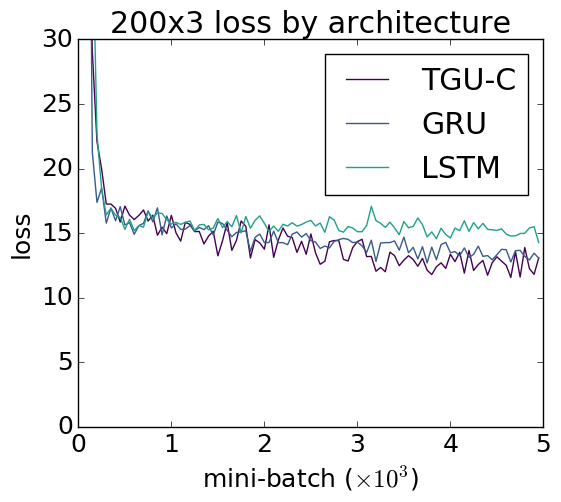
\includegraphics[width=\linewidth]{exps/vbind/plots/200x3}
	\caption{Sequence length 200.}
\end{subfigure}~
\begin{subfigure}[t]{0.3\linewidth}
	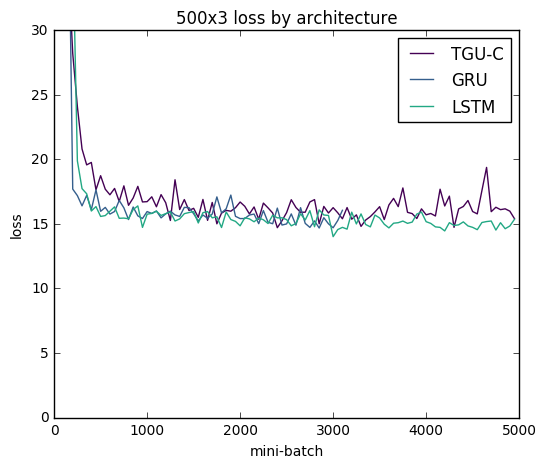
\includegraphics[width=\linewidth]{exps/vbind/plots/500x3}
	\caption{Sequence length 500.}
\end{subfigure}

\caption[Variable binding results, three patterns]
{Variable binding results for sequences containing \(3\) patterns to remember. The baseline loss for this
task is 16.6355.}
\label{fig:vbindn3}
\end{figure}

With only a single pattern to remember, the TGU dramatically outperformed the other
architectures. The LSTM was the most consistent of the other architectures tested,
although in every test by the time it had begun to escape from the baseline the TGU
had already converged. The GRU was able to make surprisingly little progress on this
task.

Increasing the number of items to remember, even just to two, makes the
task considerably harder. This highlights an issue with the manner
in which RNNs interact with their memory -- they are forced to attend to it all
at once. In a TGU where the candidate state does not
depend on the previous hidden states this requires learning a redundant mapping to embed
the input into the state-space. This is because it can not rely on the label
bits to determine which of the two inputs it is processing (this would require
access to the hidden states to determine which has switched recently). If we
assume different sets of hidden states are used to represent inputs with different
associated labels, then the candidate update must propose to update both of them
with the new input and it is up to the gate to select which update to apply.
This seems like a perfectly reasonable solution, although learning such a redundant
mapping is going to be considerably more challenging than simply learning the single
reversible transformation required to solve the task when only a single pattern
is to be remembered.

With two patterns to remember the TGU still makes the most progress 
below the baseline in the time allotted.
On the longer sequences progress is limited and none of the architectures
are close to converging although the TGU is the only architecture to
make notable progress.

When the number of patterns is increased to three all the architectures struggle.
With a sequence length of 100, there is some separation -- the TGU makes the most
progress although the GRU and LSTM also begin to progress beyond the baseline.
On the longer sequences, there is less of a clear result and when the sequence
length is 500 no models were capable of surpassing the baseline even when
allowed to train for significantly longer than reported in figure~\ref{fig:vbindn3}.

These results affirm that the TGU is competitive with the state of the art approaches.
They also suggest that the fundamental change -- focusing the expressive power in the
gate rather than the candidate update -- makes a fundamental
difference to the manner in which the network attends to its state. This change is clearly
beneficial in this task, which is highly encouraging.


\subsection{Sequential MNIST}
A pair of recently proposed tasks which have gathered significant popularity lately
are based around attempting to classify the MNIST handwritten image dataset 
\autocite{Lecun1998}. To turn two dimensional images into sequences they are
flattened in one of two ways: either in scan-line order beginning from the top-left
going one row at a time or simply by taking a random permutation \autocite{Le2015}.

This gives two tasks in which the input is a one dimensional time series to be
classified. The MNIST digits are 28 by 28 digits, so the input sequences are
784 steps long. As the majority of the pixels are black with the activity focused
in the central region, the majority of the information in the scan-line version
is focused in the middle. Contrastingly, taking a random permutation of the indices
is highly likely to induce very long time dependencies, in addition to removing
any temporal correlations in the sequence by destroying the morphology. Consequently
the permuted version is significantly more challenging. We group these with the
synthetic problems because they are somewhat arbitrary and unnatural.

Although this has been widely used recently to benchmark architectural
advances in RNNs (see, for example 
\autocite{Zhang2016, Barone2016, Gao2016, Neyshabur2016, Cooijmans2016}
solely from 2016), we argue that it does not necessarily provide a useful test of
a model's capabilities. We show this by achieving excellent performance
on the more challenging permuted task with a models which fail miserably
in real world applications. 

%This is achieved by exploiting the fact
%that although the permutation introduces artificially long time dependencies
%the underlying data is very simple -- a simple k-Nearest Neighbour classifier
%achieves 95\% accuracy \autocite{Lecun1998}. Combining the simplicity of the
%class boundaries with the sparsity of the representation in pixel-space and 
%it should be possible to succeed simply by accumulating information
%over the sequence, building a compressed representation which is then classified
%at the final time step.

\subsubsection{Proposed Architecture}
We propose an architecture specifically for this task which is a variant on
GMR proposed earlier, modified to allow for direct accumulation.
Further, we enforce this accumulative behaviour by applying a linear rectifier
to the state update. The hidden states are computed by:
\begin{equation}\label{eq:cpplus}
	\vec{h}_t = \vec{h}_{t-1} + \rho\left( \tran{\vec{x}}_t\tensor{W}\vec{h}_{t-1} + \mat{U}\vec{x}_t + \vec{b}\right).
\end{equation} This architecture should fail -- the gradients are almost
guaranteed to explode during back-propagation by the argument in section~\ref{sec:additive},
it can never remove information from its states (the state updates must be non-negative).
The only way it can make a context-dependent decision to ignore certain inputs is
if the tensor product is able to outweigh the rest of the calculation before the
non-linearity and force it to be negative. As we implement the tensor product
using a tensor in the CP decomposition, we refer to this architecture as the
``CP+''.
%
%Despite its clear shortcomings, this model achieves remarkable success on the
%sequential MNIST tasks. As discussed above we believe this is due to shortcomings
%with the task rather than special properties of the above model, as the above
%model is clearly very limited.

A model which seems slightly less absurd allows \emph{subtractive} forgetting:
\begin{align}\label{eq:cpdelta}
	\vec{a}_t &= \rho\left(\tran{\tilde{\vec{x}}}_t\widetilde{\tensor{W}}_a\tilde{\vec{y}}\right)\\
	\vec{b}_t &= \rho\left(\tran{\tilde{\vec{x}}}_t\widetilde{\tensor{W}}_b\tilde{\vec{y}}\right)\\
	\vec{h}_t &= \vec{h}_{t-1} + \vec{a}_t - \vec{b}_t.
\end{align} We denote this architecture ``CP-\(\Delta\)'' and consider only the variant in
which the bias matrices are incorporated into the tensor decomposition to keep the number
of parameters comparable. It appears more sensible
than the CP+ as it at least allows for the possibility of a negative state update.
However, this model will suffer from the same gradient issues as the CP+, although
they might be expected to be less pronounced. In practice, we find this is not the case and
the model requires at least as much guidance as the CP+.

To enable training of this model we re-parameterise the weight matrices with a
form of \emph{weight normalisation} \autocite{Salimans2016a}. Typical
weight normalisation learns unconstrained weights but applies a differentiable
normalisation transformation before use. Salimans and Kingma normalise each
row of the weight matrices to have an \(l2\) norm of \(1\), we achieved
best results by dividing each matrix by its Frobenius norm.\footnote{
For a \(n \times m\) matrix \(\mat{U}\), the Frobenius norm is
\(||\mat{U}||_F = \sqrt{\sum_i^n\sum_j^mU_{ij}^2} = ||\vect(\mat{U})||_2\).}
Back-propagation proceeds as usual through the transformation.

\subsubsection{Experiment Setup}
We are primarily concerned with the permuted task as all models tested apart
from the Vanilla RNN and GMR achieved \(98\%\) (\(\pm 1.0\)) on the simpler task.
Learning rate and rank
were found using grid-search. We train using ADAM with a batch size of 100.
For nearly all models, severe gradient clipping \autocite{Pascanu2013} is
required to train successfully, the best threshold was also found using grid
search.
Following \autocite{Le2015} all models tested have a single hidden layer of 100 units.
We use a grid search to find the best rank for the tensor models.

\subsubsection{Results}

\begin{table}
\centering
\begin{tabu} to \textwidth {r||l}
Architecture & Test Accuracy (\%)\\
\hline
TGU & 88.2\\
CP+ & 84.7\\
CP-\(\Delta\) & 91.5\\
IRNN (ours) & 84.0\\
LSTM (ours) & 86.3\\
Vanilla (ours) & 79.3\\
\hline
\emph{i}RNN \autocite{Le2015} & 82.0 \\
\emph{u}RNN \autocite{Arjovsky2015} & 91.4 \\
\emph{s}TANH-RNN \autocite{Zhang2016} & 94.0 \\
BN-LSTM \autocite{Cooijmans2016} &\textbf{95.4}\\
\hline
\end{tabu}

\caption{Test accuracy for permuted sequential MNIST.}
\label{tab:pmnist}
\end{table}

Test accuracy for the best models is reported in table~\ref{tab:pmnist}
which also includes some recent results, all
of which were state-of-the-art at the time of their publication.
Our models sit
in the middle of these results. 
This is remarkable as the 
best performing architecture, the CP-\(\Delta\) has fundamental
design flaws which cause it to fail on any other dataset we attempted
to train it on.


\begin{figure}[ht]
\centering
\begin{subfigure}[t]{0.45\textwidth}
	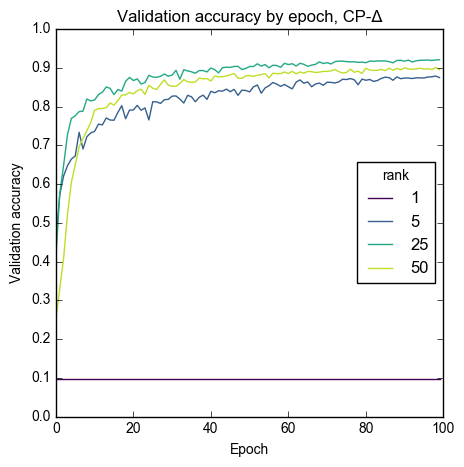
\includegraphics[width=\textwidth]{exps/mnist/cp-del-rank}
	\caption{CP-\(\Delta\) by rank}
\end{subfigure}\hfill
\begin{subfigure}[t]{0.45\textwidth}
	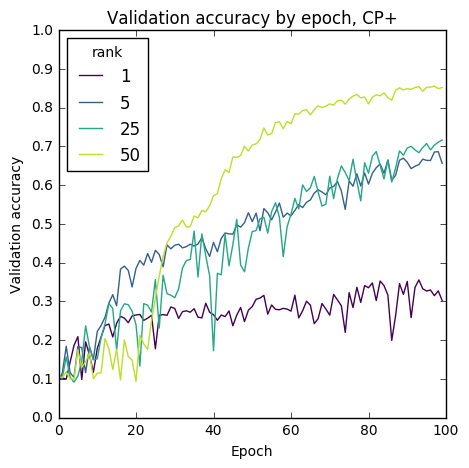
\includegraphics[width=\textwidth]{exps/mnist/cp+rank}
	\caption{CP+ by rank}
	\label{fig:cp+rank}
\end{subfigure}\\
\begin{subfigure}[t]{0.45\textwidth}
	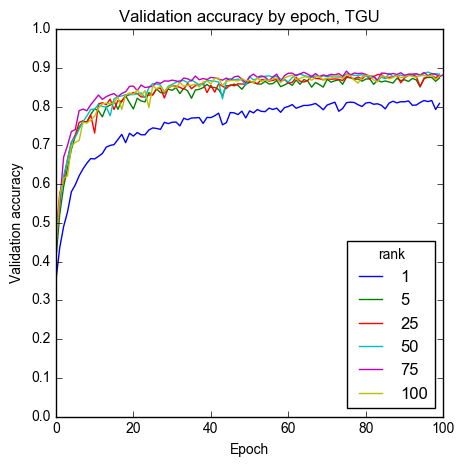
\includegraphics[width=\textwidth]{exps/mnist/tgurank}
	\caption{TGU by rank}
\end{subfigure}\hfill
\begin{subfigure}[t]{0.45\textwidth}
	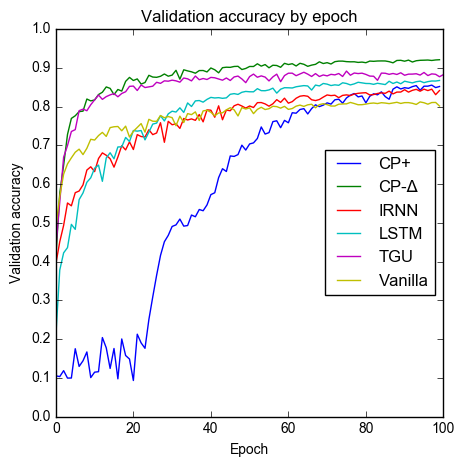
\includegraphics[width=\textwidth]{exps/mnist/allarchs}
	\caption{All architectures}
\end{subfigure}

\caption[Permuted MNIST results]{Performance (classification accuracy, \%)
 on the validation set of permuted MNIST
by rank of tensor decomposition.}
\label{fig:pmnist}
\end{figure}


Figure~\ref{fig:pmnist} shows how the performance scales with rank of
the tensor decomposition. As the CP-\(\Delta\) incorporates the
bias matrices into the decomposition, reducing the rank should greatly
affect performance. Indeed, with a rank 1 decomposition the model is
incapable of learning anything. What is more curious is that the
best performing model is not the highest rank. None of the models
had overfitting problems, we can only hypothesise that reducing the rank
might restrict the space of feasible solutions helping gradient descent.

The absurdity of the CP+ unit is clear from figure~\ref{fig:cp+rank} --
it trains in an incredibly volatile fashion. That the rank 1 model learns
at all is remarkable. The tensor product in this unit is severely
restricted, the vast majority of its learning power resides in a
feed-forward connection. This goes some way to affirming our suspicions
about this task -- although it exhibits long time dependencies, it
is almost enough to simply accumulate over all inputs.

\section{Real-world Data}
We now move on to more realistic datasets. All of the following tasks are
\emph{next-step prediction} tasks -- the goal of the network is to estimate
the probability of the next item in the sequence given the sequence so far:
\begin{equation} \label{eq:seqprob}
	p(\vec{x}_{t+1} | \vec{x}_{1},\ldots,\vec{x}_{t}).
\end{equation} The output layer of the RNN then has the task of converting
the hidden states into probabilities and so requires an appropriate non-linearity.
Training proceeds by maximising the log-likelihood of the data producing the
correct distribution.

This means that the target sequence is the input
sequence shifted across by one. If we prepend a special \emph{start-of-sequence}
symbol to the data sequence and append an \emph{end-of-sequence} symbol,
then the inputs to the network are simply all but the \emph{end-of-sequence}
and the outputs are all but the \emph{start-of-sequence}.
The end result is a statistical model of the sequence, approximating the
conditional distribution described above.
%We can sample from it
%by simply feeding it the \emph{start-of-sequence} character and then repeatedly
%sampling from the distribution generated by the current hidden states and
%feeding the sample back in to the network. This can be an interesting way to
%produce novel sequences \autocite{Graves2013}.

In all cases the data is split into three sets: training, test and validation.
The validation set is used to monitor generalisation performance and to stop
training when the model begins to overfit. We do this by checking the loss on
the validation set after each epoch. If performance has improved,
we save a checkpoint containing the model parameters. After having trained for
a fixed number of epochs the best saved model is loaded and
evaluated on the test set.

The aim of this section is not to achieve state-of-the-art performance on
large datasets. Rather we seek to ascertain whether the
theoretical reasoning and intuitions developed in the preceding chapters hold
in a more realistic setting. These datasets are less pathological than
those previously evaluated on, so it is interesting to see if the benefits
of our architectures hold in such a setting.

\subsection{Polyphonic Music}
This task, introduced by 
\autocite{Boulanger-Lewandowski2012} consists of modelling four datasets of
polyphonic music from a score. This is potentially a challenging task -- not
only do the melodies and chord progression exhibit long time dependencies, the
networks must learn the rules of harmony to produce appropriately consonant
arrangements. The likelihood of a given note at a given time step is affected
by both simultaneous information (which other notes are one at the same time)
and long term information (such as which key the piece is in). Modelling accurately
both these dependencies is challenging but reflects well the difficulties inherent
int much naturally generated data.



\subsubsection{Task}
The four datasets are:
\begin{description}
\item[Pianomidi] {
	is a collection of classical piano scores originally sourced from
	\url{http://piano-midi.de}. We split the data according to
	\autocite{Poliner2007}. This data uses the full range of the piano,
	there are 88 distinct notes present although the polyphony is limited
	as the pieces must all be played by a human.}
\item[Nottingham] {
	is a set of folk tunes converted to MIDI by 
	\autocite{Boulanger-Lewandowski2012},\footnote{
	The originals are available at: \url{http://ifdo.ca/~seymour/nottingham/nottingham.html}}
	we use their split of the data. These tunes have the simplest structure and are
	generally quite short although they span a range of 63 distinct notes.}
\item[Muse] {
	comes originally from \url{http://www.musedata.org} and contains both orchestral and
	piano classical music. This dataset has a range of 84 distinct notes and due to the
	orchestral nature of many of the scores the polyphony can be quite high. Again we
	split the data according to \autocite{Boulanger-Lewandowski2012}.}
\item[JSB] {
	consists of 382 chorales harmonised by J. S. Bach. This dataset has some of the
	lowest polyphony, as it is written in four part harmony.
	This dataset also has the smallest range of 54 notes.
	We use the split of the data given in \autocite{Allan2004}.}
\end{description} The goal of the task is to learn the conditional
distribution over notes at the current time, given the preceding sequence of notes.


\subsubsection{Experiments}
The data is converted from MIDI files (which contain note on/off events) to
an appropriate format by sampling the notes present at regular time intervals.
This gives binary vectors in which each element indicates with a one or a zero whether
a particular note is active or not.\footnote{Appropriately pre-processed data can
be downloaded from \url{http://www-etud.iro.umontreal.ca/~boulanni/icml2012}
courtesy of Boulanger-Lewandowski et al. \autocite{Boulanger-Lewandowski2012}.}
For each dataset, we fix the size of these vectors to the range of notes present in the
dataset.

Previous work is slightly inconsistent with the size of these vectors. Of those that
report it, \autocite{Boulanger-Lewandowski2012} fix the size of the vectors for all
datasets to the range of 88 notes available on a piano while \autocite{Chung2014}
use much larger vectors although it is not clear why. We fix the size of the
inputs to the range of the notes present in the data. As the data is
written for specific instruments it only makes sense to train the model to attend
to an appropriate range for those instruments. This means
results can not be directly compared although they are very similar,
with nearly all of our RNNs surpassing \autocite{Chung2014} and achieving performance
similar to the RNNs evaluated in \autocite{Boulanger-Lewandowski2012}. We would
expect our RNNs to report slightly higher negative log-likelihoods as we use input/output
sizes with no redundancy -- there are no outputs the network can learn to switch off
constantly bringing down the average loss.
Further, the more unexpected elements of the results such as the performance of the
Vanilla RNN on Nottingham are present in others' results.

All networks used a single hidden layer. The number of hidden nodes and the rank of
the tensor decomposition was chosen so that each network would have as close to
20,000 parameters when applied to the JSB dataset as possible. This was done 
so that the comparison is not skewed by models such as
the LSTM which have a large number of parameters per hidden unit. The rank was set as
either \(1\) or a multiple of the number of hidden states, chosen from \(\{1/2, 1, 2\}\).
Table~\ref{tab:jsbsizes} in the appendix shows the number of hidden units and the rank of the tensor
decomposition for the models evaluated. The networks used a sigmoid output layer to
appropriately model the fact that the multiple output units may need to be on at once.


A preliminary grid search was undertaken on a subset of the architectures to determine
sensible ranges for the final experiments. Models reported were trained using ADAM with
a grid search over the following hyper-parameters: base learning rate from \(\{0.01, 0.001\}\),
maximum length of back-propagation through time chosen from \(\{75, 100\}\) steps
and rank as discussed above. The batch size was set to \(8\). For nearly all architectures 
best performance was
achieved with the lower learning rate while the best maximum length was task-dependent.

\subsubsection{Results}
%\begin{table}
%\begin{tabu} to \linewidth {r||c|c|c}
%\hline
%		 \multicolumn{4}{c}{Nottingham} \\
%    	& \emph{Train}      & \emph{Valid}    & \emph{Test} \\
%\hline
%Vanilla   & \textbf{3.3278} & 3.8680 & \textbf{3.8871}      \\ % sl 100
%LSTM      & 3.5826          & 3.9683          & 4.0124		\\ % sl 100
%GRU		  & 3.5876		    & 3.9871		  & 4.0157		\\ % sl 100
%GMR	  & 3.3940		    & \textbf{3.8472} & 3.9055		\\ % rankone sl 100
%GMR-C   & 3.7902		    & 4.1242          & 4.1350		\\ % rankhalf sl 75
%TGU		  & 3.9652		    & 4.2069          & 4.2140		\\ % rankone sl100
%TGU-C     & 4.0035		    & 4.2332	      & 4.2531		\\ % rankfull sl100
%lin-TGU   & 3.9387		    & 4.2095	      & 4.2255		\\ % rankone sl 75
%lin-TGU-C & 3.9927		    & 4.2726          & 4.2907\\ % rankhalf sl 100
%\hline\hline
% \multicolumn{4}{c}{JSB} \\
%    	& \emph{Train} & \emph{Valid} & \emph{Test} \\
%\hline
%Vanilla   & 8.0284	        & 8.5417	      & 8.6381   \\ % sl 75
%LSTM      & 8.2058	        & 8.5444	      & 8.6633   \\ % sl 75
%GRU		  & 8.1689	        & 8.5657	      & 8.6027   \\ % sl 75
%GMR	  & 8.0526	        & 8.5465	      & 8.6084   \\ % rankone sl 75
%GMR-C   & 8.0093	        & \textbf{8.4656} & 8.5369   \\ % rankhalf sl 100
%TGU		  & \textbf{7.9357} & 8.5140	      & 8.6060   \\ % rankhalf sl 75
%TGU-C     & 7.9731	        & 8.4926	      & \textbf{8.5307}   \\ % rankone sl 100
%lin-TGU   & 8.0645	        & 8.7126	      & 8.7282   \\ % rankhalf sl 75
%lin-TGU-C & 8.2257	        & 8.6549	      & 8.7117   \\ % rankhalf sl 100
%\hline\hline
% \multicolumn{4}{c}{Pianomidi} \\
%    	& \emph{Train} & \emph{Valid} & \emph{Test} \\
%\hline
%Vanilla   & 7.3874	        & 8.5956	      & 7.8093   \\ % sl 75
%LSTM      & 7.3730	        & \textbf{8.5329} & 7.7542   \\ % sl 75
%GRU		  & 7.3039	        & 8.5671	      & 7.7652   \\ % sl 100
%GMR	  & 7.3598	        & 8.5890	      & 7.7676   \\ % rankone sl 100
%GMR-C   & 7.4244	        & 8.7350	      & 7.8615   \\ % rankhalf sl 100
%TGU		  & \textbf{7.2132} & 8.5981	      & 7.7161   \\ % rankhalf sl 100
%TGU-C     & 7.2748	        & 8.5382	      & \textbf{7.7003}  \\ % rankhalf sl 75
%lin-TGU   & 7.2866	        & 8.5807	      & 7.7475   \\ % rankhalf sl 75
%lin-TGU-C & 7.3216	        & 8.5716	      & 7.7209   \\ % rankhalf sl 75
%\hline\hline
% \multicolumn{4}{c}{Muse} \\
%    	& \emph{Train} & \emph{Valid} & \emph{Test} \\
%\hline
%Vanilla   & 6.8954	        & 7.2597	      & 7.3619   \\ % sl 100
%LSTM      & 7.0777	        & 7.3652	      & 7.4159   \\ % sl 75
%GRU		  & 7.0001	        & 7.3256	      & 7.3824   \\ % sl 100
%GMR	  & \textbf{6.8864} & \textbf{7.2089} & \textbf{7.3089}   \\ % rankone sl 100
%GMR-C   & 6.9135	        & 7.3349	      & 7.4296   \\ % rankfull sl 100
%TGU		  & 7.4524	        & 7.7076	      & 7.6879   \\ % rankone sl 100
%TGU-C     & 7.4551	        & 7.6842	      & 7.6719   \\ % rankhalf sl 100
%lin-TGU   & 7.5478	        & 7.7732	      & 7.7428   \\ % rankhalf sl 75
%lin-TGU-C & 7.6134	        & 7.8147	      & 7.7949   \\ % rankfull sl 75
%\hline
%\end{tabu}

\begin{table}
\centering
\begin{tabu} to \linewidth {r||c|c||c|c||c|c||c|c|}
%\hline
	&	 \multicolumn{2}{c||}{Nottingham}     & \multicolumn{2}{c||}{JSB}          & \multicolumn{2}{c||}{Pianomidi}   & \multicolumn{2}{c}{Muse} \\
    	& \emph{Train}     & \emph{Test}      & \emph{Train}    & \emph{Test}      & \emph{Train}    & \emph{Test}     & \emph{Train}    & \emph{Test} \\
\hline
GMR	      & 3.3940		   & 3.9055		      & 8.0526	        & 8.6084           & 7.3598	         & 7.7676          & \textbf{6.8864}& \textbf{7.3089}\\
GMR-C     & 3.7902		   & 4.1350		      & 8.0093	        & 8.5369           & 7.4244	         & 7.8615          & 6.9135	        & 7.4296 \\
TGU		  & 3.9652		   & 4.2140		      & \textbf{7.9357} & 8.6060           & \textbf{7.2132} & 7.7161          & 7.4524	        & 7.6879 \\
TGU-C     & 4.0035	       & 4.2531		      & 7.9731	        & \textbf{8.5307}  & 7.2748	         & \textbf{7.7003} & 7.4551	        & 7.6719   \\
\hline
Vanilla   & \textbf{3.3278}& \textbf{3.8871}  & 8.0284	        & 8.6381           & 7.3874	         & 7.8093          & 6.8954	        & 7.3619   \\    
LSTM      & 3.5826         & 4.0124		      & 8.2058	        & 8.6633           & 7.3730	         & 7.7542          & 7.0777	        & 7.4159   \\ 
GRU		  & 3.5876		   & 4.0157		      & 8.1689	        & 8.6027           & 7.3039	         & 7.7652          & 7.0001	        & 7.3824   \\
\hline
% \multicolumn{4}{c}{Muse} \\
%    	& \emph{Train} & \emph{Valid} & \emph{Test} \\
%\hline
%Vanilla   & 6.8954	        & 7.2597	      & 7.3619   \\ % sl 100
%LSTM      & 7.0777	        & 7.3652	      & 7.4159   \\ % sl 75
%GRU		  & 7.0001	        & 7.3256	      & 7.3824   \\ % sl 100
%GMR	  & \textbf{6.8864} & \textbf{7.2089} & \textbf{7.3089}   \\ % rankone sl 100
%GMR-C   & 6.9135	        & 7.3349	      & 7.4296   \\ % rankfull sl 100
%TGU		  & 7.4524	        & 7.7076	      & 7.6879   \\ % rankone sl 100
%TGU-C     & 7.4551	        & 7.6842	      & 7.6719   \\ % rankhalf sl 100
%\hline
\end{tabu}

\caption[Polyphonic music modelling results]
{Results on polyphonic music datasets. Numbers are average negative log-likelihood, lower is better.
 ``-C'' appended to the tensor units indicates the bias matrices are folded into the decomposition,
 otherwise they are separate.}
\label{tab:jsbresults}
\end{table}

Results for the four datasets are found in table~\ref{tab:jsbresults}. We report the average
negative log-likelihood the best early-stopped models assign the data vectors over
the training, test and validation sets.

In general the tensor units performed better than their counterparts except on
Nottingham, the simplest of the datasets. This dataset consists of folk songs which
are often very formulaic in their harmony. Correspondingly, simple models seem to be able to
perform very well. It also seems to be the case that there is something about the structure
of the data which suits the Vanilla RNN -- the best GMR (which was the closest to the
Vanilla RNN out of all architectures) had a rank \(1\) tensor decomposition meaning
that it was functionally nearly identical to a Vanilla RNN.

In fact, all of the best GMR models used a rank 1 tensor decomposition. This is interesting
as it suggests the extra complication of the tensor product only hindered learning.
Alternatively, it may be that it is beneficial to have more
hidden units even if that comes at the cost of decreased representational power. This effect
was only notable in the GMR. 

Interestingly the TGU-C models generally outperformed their counterpart TGUs on the test data but
not on the training data. This suggests that having the ability to constrain the representative
power of the gate can provide a useful regularising effect.

\subsection{PTB}
The next experiment tests whether reducing the number of parameters in the model by lowering
the rank of the tensor decomposition can have a regularising effect. For this we use the
Penn Treebank \autocite{Marcus1993} and attempt to model it by word using the next-step prediction
framework outlined earlier. This is a relatively small dataset and overfitting becomes a serious
challenge. Due to this the dataset has been popular for testing regularisation approaches for
recurrent neural networks \autocite{Zaremba2014, Gal2015}.

We are concerned with how the tensor that computes the gate values in the TGU affects the ability of
the network to make use of its memory. To test this we fix the number of hidden units and vary the
rank of the tensor.

\subsubsection{Experiment Setup}
The data is pre-processed following \autocite{Zaremba2014} by replacing all but the most common
10,000 words with an `unknown' symbol. We train using ADAM with a batch size of 20. Base learning
rate for each model was found via grid search.
All networks trained had 128 hidden units -- for this experiment we do not attempt to keep the number
of trainable parameters equal between models. We test four variations of the TGU: with and without
combined biases with with linear or rectified linear candidate updates. For comparison we also train
an LSTM, GRU and Vanilla RNN. The GMR performed unremarkably on this data, so we omit it from our
results.

\subsubsection{Results}
For this task we report the average word-level perplexity over the test set. The perplexity is the 
exponentiation of the cross entropy between the predicted distribution and the target distribution
(lower is better).

Overall results are
presented in table~\ref{tab:ptb}. The best performance across all models was achieved by the TGU with
linear candidate updates and separate biases. Three out of four of the TGUs surpassed the LSTM with
linear candidate updates having a clear advantage.

\begin{table}
\centering
\begin{tabu} to \textwidth {r||l|l|l}
 Architecture (rank) & \emph{Train} & \emph{Valid} & \emph{Test} \\
\hline
TGU   (64)    & 82.86 & 139.54 & 131.42 \\
TGU-C  (64)   & 92.73 & 147.90 & 139.15 \\
lin-TGU (64)  & 91.81 & 127.80 & \textbf{121.93} \\
lin-TGU-C (128) & 99.74 & 133.77 & 127.56 \\
\hline
LSTM      & \textbf{78.74} & 144.75 & 134.79 \\
GRU       & 79.89 & \textbf{133.55} & 127.56 \\
Vanilla   & 85.10 & 164.81 & 156.63 \\
\hline
\end{tabu}

\caption[PTB test set results]{Per-word perplexity of best early-stopped models on the Penn Treebank test set.}
\label{tab:ptb}
\end{table}


\begin{figure}[ht]
\centering
\begin{subfigure}[t]{0.45\textwidth}
	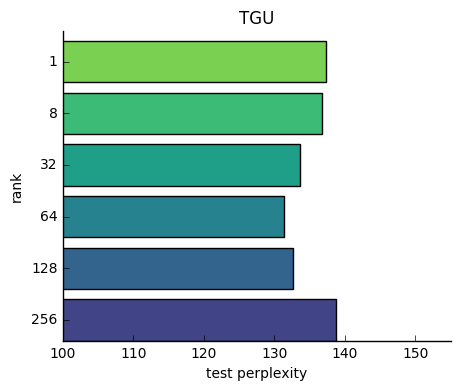
\includegraphics[width=\textwidth]{exps/ptb/tgu-rank}
\end{subfigure}\hfill
\begin{subfigure}[t]{0.45\textwidth}
	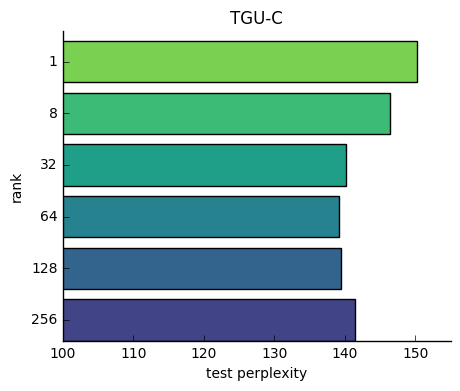
\includegraphics[width=\textwidth]{exps/ptb/tguc-rank}
\end{subfigure}\\
\begin{subfigure}[t]{0.45\textwidth}
	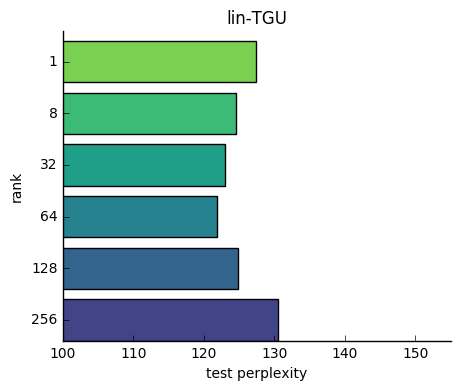
\includegraphics[width=\textwidth]{exps/ptb/lintgu-rank}
\end{subfigure}\hfill
\begin{subfigure}[t]{0.45\textwidth}
	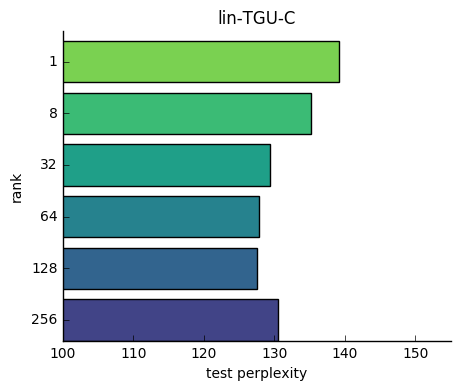
\includegraphics[width=\textwidth]{exps/ptb/lintguc-rank}
\end{subfigure}

\caption[TGU PTB results by rank]{Test perplexity
 of best early stopped models for
each type of TGU for a range of ranks. Networks had 128 hidden units.}
\label{fig:ptbtgurank}
\end{figure}


Figure~\ref{fig:ptbtgurank} shows results of the TGUs organised by rank. For all models there
is a clear benefit to constraining the tensor to half the number of hidden states. When the biases
are combined the difference between rank 64 and 128 is less clear cut, which is to be expected as
the expressive power of the tensor unit is much more constrained by the rank. That none of the models
with separate biases improve performance with a rank below 64 indicates that the tensor is performing
a valuable role as robbing it of power harms performance.


\subsection{War and Peace}
We perform one final experiment to test whether the regularising effect
observed so far are due to limiting the expressive power of the tensor
or simply reducing the parameters. We do this by adjusting the number of hidden units so that
all models have the same number of trainable parameters regardless of rank.

As data for this test we use the novel War and Peace by Leo Tolstoy to build character level language
models. This is mostly in English and in order to succeed the models must learn to model long term
temporal dependencies such as opening and closing quotations marks, correct punctuation and grammar
as well as higher level language concepts.

\subsubsection{Experiment Setup}
Experiments are set up very similarly to \autocite{Karpathy2016}. Accordingly we split the 3,258,246
characters into training/validation/test sets with an 80/10/10 \% ratio, giving approximately
300,000 characters in the training and validation sets. The book contained a vocabulary of 83 characters.
Again we train using ADAM, we found a learning rate of 0.001 to be robust for all models. We use a
batch size of 100 and limit back-propagation of gradients to 100 steps. Models were trained for
50 epochs at most.

We found even very small models overfit dramatically even after one or two epochs. To approach
reasonable baseline performance, we introduce a bottleneck before the network in the form of very
small character embeddings. This is equivalent to encoding the input symbols as one-hot vectors
(size \(83 \times 1\)) and multiplying by a \(8 \times 83\) matrix to embed the symbols into an
8 dimensional space. This matrix is learned jointly with the model and has dropout 
\autocite{Srivastava2014} applied to further prevent overfitting.

Models were constrained to have a budget of 25,000 parameters (including the output layer but
not including the embedding matrix). This corresponds to
an LSTM with 65 hidden units. The rank one GMR with combined 
biases, by contrast,
was able to have 293 hidden units, although it proved incapable of making use of the them. Vanilla RNNs
perform well on this task, so we test the GMR in addition to the TGU. As we are interested
in the effect of low-rank tensor decompositions on expressive power, we only report results for models
with combined biases to exacerbate the effects.
We found linear candidate activations consistently outperformed rectifiers for
the TGU.
Rank was chosen in the same way as the polyphonic music experiment, although we allow ranks as low as
a quarter of the number of hidden units.

\subsubsection{Results}
\begin{figure}
\centering
\begin{subfigure}[t]{0.3\textwidth}
	\centering
	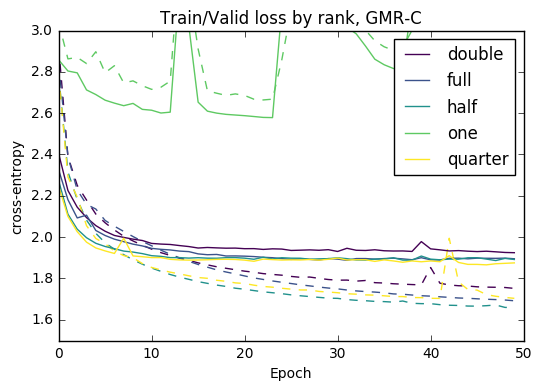
\includegraphics[width=\textwidth]{exps/wp/gmr}
	\caption[War and Peace, GMR]
	{GMR-C by relative rank.}
\end{subfigure}~
\begin{subfigure}[t]{0.3\textwidth}
	\centering
	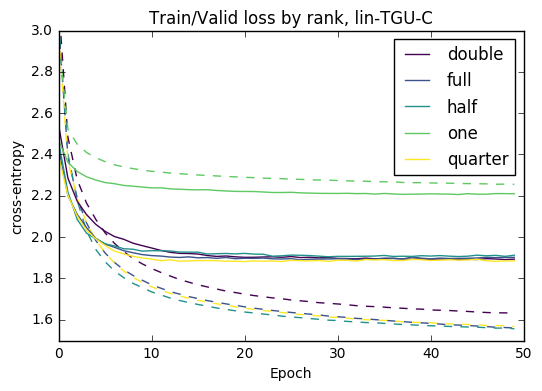
\includegraphics[width=\textwidth]{exps/wp/lintgu}
	\caption[War and Peace, TGU]
	{TGU-C (with linear candidate states) by relative rank.}
\end{subfigure}~
\begin{subfigure}[t]{0.3\textwidth}
	\centering
	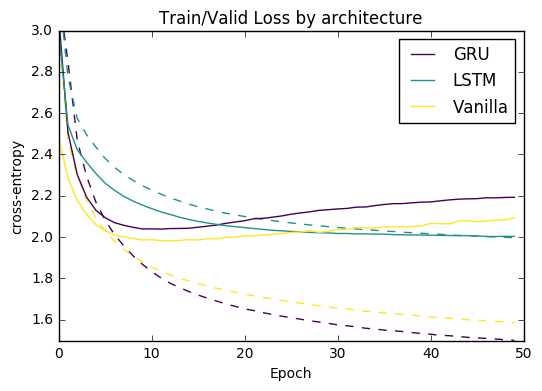
\includegraphics[width=\textwidth]{exps/wp/others}
	\caption[War and Peace, other architectures]
	{Other architectures exhibit slow learning or dramatic overfitting.}
\end{subfigure}~
\caption[War and Peace, training curves]
		{Training and validation curves on War and Peace. 
		 Dashed lines indicate training loss, solid lines are the loss on the validation set.
		 `Full' refers to rank equal to the number of hidden units, `one' simply means rank 1.}
\label{fig:wp}
\end{figure}

Training and validation cross entropy are plotted in figure~\ref{fig:wp}. 
The tensor models both
show remarkable resistance to overfitting compared to the other architectures. What is particularly
interesting is that the validation error does not begin to rise seriously at all, regardless of the
rank. Aside from rank one, which struggles to learn at all, the models benefit slightly from lower
rank with best test performance being achieved by both tensor models with rank equal to a quarter
of their number of hidden units. The best GMR reported the best results on the test sets -- we
attribute this to the fact that its only component is a tensor product so altering the rank has
a much greater effect.

Perhaps more unexpectedly, even the tensor model with an excessive rank of twice the number of hidden
units still fails to overfit as dramatically as the LSTM or the Vanilla RNN. This seems to suggest that
the tensor units work particularly well with the small embeddings and dropout even though they were primarily
applied to allow the other architectures to report validation cross entropies in a reasonable range
at the end of training.

\begin{table}
\centering
\begin{tabu} to \textwidth {r||c}
Architecture & Test Cross-Entropy \\
\hline
GMR-C & \textbf{2.018} \\ % 154 width 38 rank
lin-TGU-C & 2.052 \\ % 148 width 37 rank
\hline
Vanilla & 2.128 \\ % 118 width
GRU & 2.1621 \\ % 75 width
LSTM & 2.1271 \\% 65 width
\hline
\end{tabu}
\caption{Test set cross entropy (per character) for the best War and Peace models.}
\label{tab:wptest}
\end{table}
